\section{Anatomy of a CBIR System}\label{sec:anatomy}

The inner workings of most CBIR systems can best be examined by looking at the
processing pipeline each query has to go through. The coarse sequence of
computational steps is almost the same in all such systems (Figure
\ref{fig:cbir_coarse_structure}):

\begin{enumerate}
    \item Acquire the image.
    \item Extract the signature using a feature extraction algorithm.
    \item Compare the signature to a database containing the signatures of the
        images to search within.
    \item Rank the images by similarity using the comparison results.
\end{enumerate}

\begin{figure}[h]
    \centering
    \subfloat[Local features]{%
        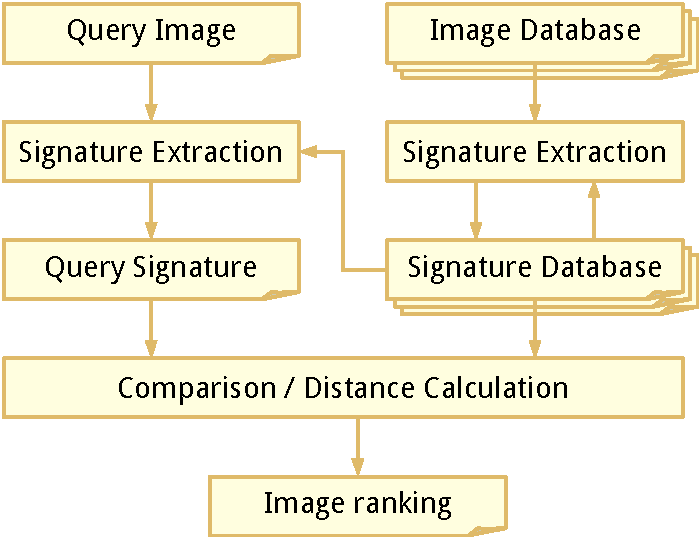
\includegraphics[width=0.45\textwidth]{cbir_anatomy_query_local_cropped}%
        \label{fig:cbir_coarse_structure_local}%
    }
    \quad
    \subfloat[Global features]{%
        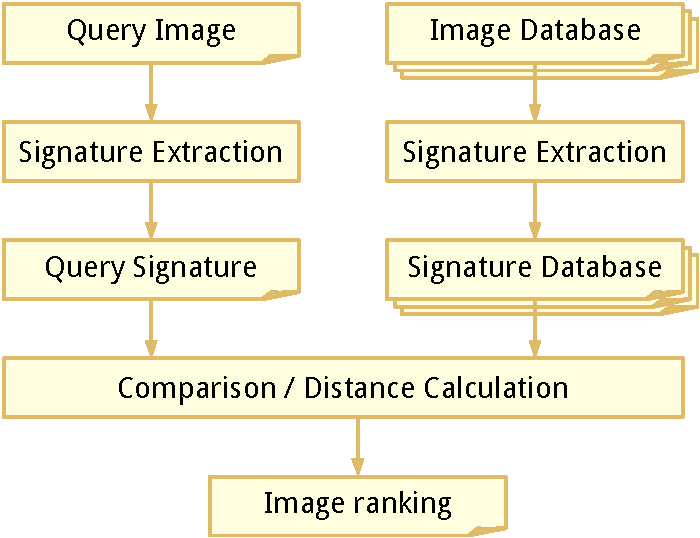
\includegraphics[width=0.45\textwidth]{cbir_anatomy_query_cropped}%
        \label{fig:cbir_coarse_structure_global}%
    }
    \caption[Coarse structure of a CBIR system]{
        The processing pipeline for CBIR using both local and global features
        is very similar. The main difference is in the signature extraction
        step, in which local features are selected, weighted and/or compressed
        depending on the results of the signature extraction of the other
        images in the database.
    }
    \label{fig:cbir_coarse_structure}
\end{figure}

\subsection{Image Acquisition}\label{sec:anatomy_image_acquisition}

The format in which the images are available to the system determines the
maximum amount of information available to subsequent analysis steps.

A significant part of the preprocessing usually done after acquisition depends
on the broadness of the image domain. The concept of the domain encompasses and
describes the variability of many possible image parameters like illumination
or composition and is therefore closely related to the sensory gap described
above. The narrower the image domain is, the more assumptions the system can
make about image from that domain. By their very nature, the domain of sketch
based image retrieval systems is usually very broad. It contains the sketches
create by the user to query the database as well as the images in the database
itself, which can be of a completely different nature, e.g.\ photos or
paintings.

Another factor usually is the accepted input format of the feature extraction
algorithm. Many algorithms like SIFT \autocite{lowe_object_1999} or SURF
\autocite{bay_speeded-up_2008} are defined for single-channel data, but some
have been specifically developed to operate on multi-channel images, like cSIFT
\autocite{abdel-hakim_csift:_2006} and \autocite{yang_robust_2008}.

\subsection{Signature Extraction}\label{sec:anatomy_signature_extraction}

The signature of an image is its representation in the following comparison
step. Therefore it should describe the image using its most discriminatory
features compared to all other images in the database. Due to the effects of
the \emph{sensory gap} discussed above, there is, at the moment, no definitive
way to determine the discriminatory power of features in general, even though
knowledge about the image domain can guide the descisions.  The signature
composition depends on both, the kind of features extracted from the image and
the way these features are encoded. 

Over the last two decades, a wide variety of feature descriptors have been
published, which mostly focus on specific types of features. Some techniques
use color histograms \autocite{utenpattanant_color_2006}, while others
\autocite{stricker_color_1996} \autocite{deng_efficient_2001}
\autocite{lee_spatial_2003} include spatial relations between colors in a
region.
Many descriptors attempt to capture texture characteristics, such as
\autocite{schaffalitzky_viewpoint_2001} and \autocite{manjunath_texture_1996}.
Rubner and Thomasi \autocite{rubner_texture-based_1999} combine Gabor filters
and the earth mover's distance and thereby bypass segmentation.
Another class of descriptors focuses on representing shapes using detection of
edges and salient points. Lowe \autocite{lowe_object_1999} developed the now
widely adopted SIFT descriptor, that employs clustering of salient points. More
recently, the SURF desciptor \autocite{bay_speeded-up_2008} uses Haar wavelets
to deliver comparable performance.
Several publications combine feature types to arrive at a more comprehensive
descriptor. Oliva and Torralba \autocite{oliva_modeling_2001} capture various
scene properties like "roughness" and "openness".

\begin{figure}[h]
    \centering
        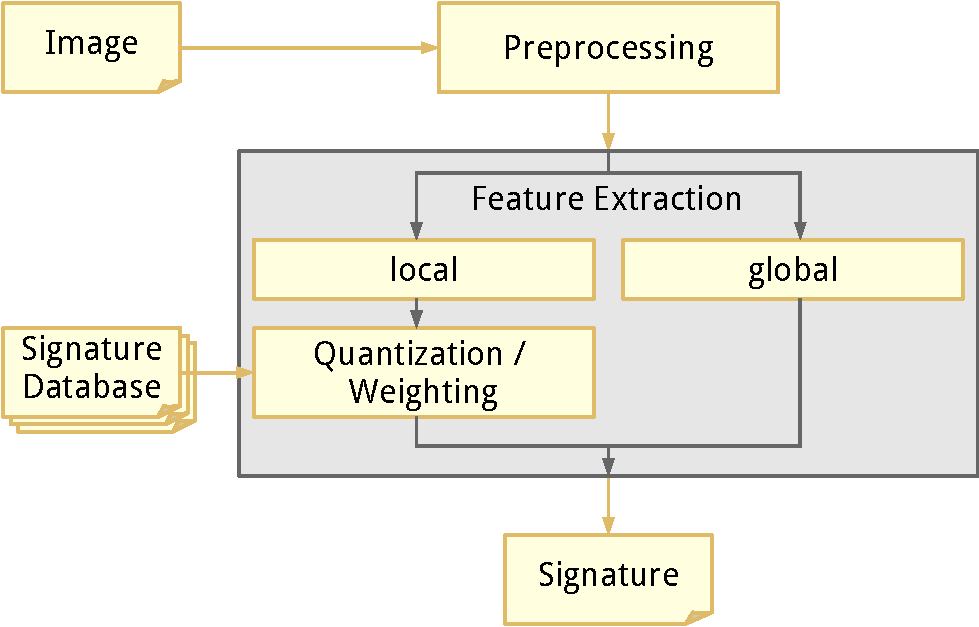
\includegraphics[width=0.8\textwidth]{cbir_anatomy_signature_extraction_cropped}
    \caption{Signature extraction in CBIR systems}
    \label{fig:cbir_signature_extraction}
\end{figure}

\subsubsection{Global Features}

Aside from the nature of the features captured by a descriptor, there are also
differences in the geometrical scope the features are derived from. Global
feature descriptors attempt to capture the structure of the whole scene or
describe the distribution of properties across the image like the binary Haar
color descriptor published in \autocite{utenpattanant_color_2006}. Some global
algorithms subdivide the image into regular segments and derive the localized
distribution of features for each division. \autocite{lazebnik_beyond_2006}
improves upon this concept by creating feature pyramids using iterative
subdivision for multiscale analysis. While the computational complexity of
those global approaches is usually quite low, they are especially susceptible
to problems like partial occlusion or reflections within the scene. The spatial
envelope descriptor \autocite{oliva_modeling_2001} combines a global
spectrogram with locally derived spectral information to produce an overall
image descriptor.

\subsubsection{Local Features}

In contrast to the global approach, many CBIR systems employ "bag-of-features"
descriptors, that represent the image as an unsorted collection of local
features extracted from small patches of the image. The unsorted nature of the
feature collection leads to loss of large-scale geometric structures that can
be counteracted by a suitable choice of the patch sizes. When the local feature
descriptors are invariant to rotation, scale or similar deformations, the
sensitivity to viewpoint variations or occlusions decreases. The prominent SIFT
descriptor \autocite{lowe_object_1999} achieves this by selecting the feature
locations such that they can be normalized with respect to scale, orientation
and limited 3D projections. The SURF descriptor by Bay et al
\autocite{bay_speeded-up_2008} gives similar results, but has reduced
computational requirements. The HOG descriptor \autocite{dalal_histograms_2005}
calculates histograms of gradient directions on regular grid cells to describe
the local angular distribution of edges.

\subsubsection{Dimensionality Reduction}

The signatures produced by local descriptors are often large sets of vector,
that are themselves of considerable size. For example, the SIFT descriptor
describes each image using about $1000$ local feature vectors of $160$ values
each. Such large numbers of vectors are expensive to store and compare, so one
of several data reduction methods is commonly used.

\paragraph{Principal Component Analysis}

The Principle Component Analysis (PCA) is a transformation, that computes the
orthogonal basis best suited to describe the variance of the data. An
$n$-dimensional data set is linearly mapped to a coordinate system, in which
the direction of the first axis $a_1$ is the direction with the largest
variance in the data. The following axes' $a_i$, $i \in 2, \dots, n$ directions
correspond to the orthogonal directions with the next-largest variances in
descending order. By choosing the $p$ largest component vectors and performing
an inverse transformation of the PCA-transformed data, a projection of the
original data in $p$ dimensions can be obtained. Due to the choice of the
vectors for the inverse transformation, the projection discards only the parts
of each observation that vary the least between all observations.

PCA has been applied to the face recognition problem using intensity images
(eigenfaces) \autocite{turk_face_1991}, wavelets (waveletfaces)
\autocite{feng_human_2000} and more recently curvelets (curveletfaces)
\autocite{mandal_face_2008}. In \autocite{ke_pca-sift:_2004} it was used to
improve the robustness of the SIFT \autocite{lowe_object_1999} descriptor. To
overcome the limited between-class discrimination of PCA, it has been combined
with Linear Discriminant Analysis (LDA), yielding even better results
\autocite{mandal_curvelet_2009}.

\paragraph{Visual Words and Clustering}\label{sec:anatomy_clustering}

Instead of reducing the size of the individual feature vectors, the
bag-of-features approach collects the feature vectors into a single signature
vector to represent the image. This is done by determining a codebook of
representative feature vectors, the "visual words" \autocite{sivic_video_2003},
and assigning each local feature vector to the most similar visual word. A
histogram of the distribution of visual words can then be calculated as a
signature for each image.

To create the codebook, the large number of feature vectors extracted from
local patches of each image in the database are grouped into clusters of
similar vectors. The optimal number of clusters is usually determined
experimentally and varies with other processing parameters such as the sampling
strategy \autocite{nowak_sampling_2006} \autocite{yang_evaluating_2007}.

% k-means

The most common clusting method used in numerous publications
\autocite{zhu_theory_2002} \autocite{sivic_video_2003}
\autocite{csurka_visual_2004} \autocite{fergus_learning_2005}
\autocite{winn_object_2005} is k-means clustering. This algorithm uses the
euclidean distance as a metric to assign each observation $x_p$ to the nearest
cluster $S_i$ with mean $m_i$, $i \in 1, \dots, k$. The goal is to minimize
the variance within each cluster:
\begin{equation*}
    \sum_{i=1}^k \sum_{x_p \in S_i} \| x_p - m_i \|^2
\end{equation*}

Lloyd's algorithm is the usual way to calculate a k-means partition. It
requires a set of $k$ intial cluster centers, that are often randomly chosen
from the dataset or randomly generated. The cluster centers $m_i$ are then
iteratively adjusted until no reassignment takes place in two consecutive
iterations $t$ and $t+1$. In each iteration, each oberservation $x_i$ is
assigned to exactly one cluster $S_i$ using
\begin{equation*}
    S_{i, t} = \left\{ x_p : \| x_p - m_{i, t} \| \leq \| x_p - m_{j, t} \| \quad \forall j \in 1, \dots, k \right\}.
\end{equation*}
The centers are then recalculated as
\begin{equation*}
    m_{i, t+1} = |S_{i, t}|^{-1} \sum_{x_p \in S_{i, t}} x_p.
\end{equation*}

The greedy nature of the algorithm and the random initialization mean that it
is merely a heuristic and can converge on a local minimum, that not a global
minimum.
Other clusting methods are hierarchical agglomorative and divisive algorithms as
used in \autocite{nister_scalable_2006} and \autocite {philbin_object_2007},
that recursively divide or merge partitions to optimize the vocabulary.

Once the clustering algorithm has converged, the cluster centers $m_i$ will be
used as the visual words of the codebook. To create the signature vector of an
image, its feature vectors $x_p$ will be quantized by grouping them into sets
$S_i$, $i \in 1, \dots, k$ such that
\begin{equation*}
    S_i = \left\{ x_p : \| x_p - m_{i} \| \leq \| x_p - m_{j} \| \quad \forall j \in 1, \dots, k \right\}.
\end{equation*}
The final image signature $\tilde{I}$ then is the vector of the cardinality of these sets:
\begin{equation*}
    \tilde{I} = \big( |S_1|, |S_2|, \dots, |S_{k-1}|, |S_{k}| \big)
\end{equation*}

\subsection{Comparison and Ranking}\label{sec:anatomy_ranking}

\subsubsection{Distance Metrics}

\paragraph{Euclidean Distance}

The simplest and probably most widely used distance metric is the euclidean
distance. Its two-dimensional variant is derived from the formula of
Pythagoras. Generalized to $n$-dimensional points $p = (p_1, p_2, \dots, p_n$
and $q = (q_1, q_2, \dots, q_n)$, it can be written as
\begin{equation*}
    d_{EUCL}(p, q) = \sqrt{\sum_{i=1}^n (q_i - p_i)^2}.
\end{equation*}

\paragraph{Mahalanobis Distance}

If the distance metric is used for clustering or classification of datasets
with non-spherical within-class distributions, the euclidean distance will
naturally not perform well. A common alternative is the Mahalanobis distance,
that incorporates the correlation of the dataset into the result. The distance
of a point $p = (p_1, p_2, \dots, p_n)$ to a cluster with mean $m = (m_1, m_2,
\dots, m_n)$ is
\begin{equation*}
    d_{MAHA}(p, m) = \sqrt{(p - m)^T S^{-1} (p - m)},
\end{equation*}
where $S$ is the cluster's covariance matrix. In practice, it has been used in
\autocite{mikolajczyk_scale_2004} and \autocite{sivic_video_2003} to compare
feature vectors of the SIFT \autocite{lowe_object_1999} descriptor.

\paragraph{Cosine Distance}

A metric sometimes used in information retrieval applications is the coside
distance or cosine similarity. The similarity is defined as the cosine of the
angle between two vectors $p = (p_1, p_2, \dots, p_n$ and $q = (q_1, q_2,
\dots, q_n)$ when interpreted geometrically:
\begin{equation*}
    cos(\theta_{p, q}) = \frac{p \cdot q}{\|p\| \|q\|}
\end{equation*}
This means that the metric effectively normalizes the vectors in respect to
their euclidean length. That effect is often used in text retrieval to achieve
invariance regarding the document size.

\paragraph{Earth Mover's Distance}

The Earth Mover's Distance (EMD) is an application of the discrete
transportation problem, which was first introduced into the field of computer
vision in \autocite{peleg_unified_1989}. The use of the algorithm as a signature
comparison metric in image retrieval was published by Rubner et al.\
\autocite{rubner_metric_1998}. At the abstract level, the distance is calculated
as the amount of work necessary to transform one signature into the other.
A main advantage of the EMD over most other distance measures is that it
accounts for inter-bin distances (ground distances) in binned distributions.
Another useful property is the ability to compare distributions of different
sizes, e.g. for partial matching.
For signatures $P = \{ (p_1, w_{p_1}), \dots, (p_n, w_{p_n}) \}$ and $Q = \{
(q_1, w_{q_1}), \dots, (q_m, w_{q_m}) \}$ of bin centers $p_i$ and $q_i$ with
bin sizes $w_{p_i}$ and $w_{q_i}$ the pairwise ground distances can be
represented in a $n \times m$ matrix $D$.
These ground distances $d_{i, j}$ between two bins is then interpreted as the
costs of moving a unit of goods from one bin to the other. The optimal solution
minimizes the overall costs by finding flow values $f_{i, j}$ between each pair
$p_i$ and $q_i$, that satisfy the constraints
\begin{align*}
    f_{i, j} & \geq 0 \\
    \sum_{j=1}^m f_{i, j} & \leq w_{p_i} \\
    \sum_{i=1}^n f_{i, j} & \leq w_{q_j} \\
    \sum_{i=1}^n \sum_{j=1}^m f_{i, j} & = min \left( \sum_{i=1}^n w_{p_i}, \sum_{j=1}^m w_{q_j} \right)
\end{align*}
for all $1 \leq i \leq n$ and $1 \leq j \leq m$.
The distance between signatures $P$ and $Q$ can then be calculated as
\begin{equation*}
    d_{EMD}(P, Q) = \frac{\sum_{i=1}^n \sum_{j=1}^m d_{i, j} f_{i, j}}{\sum_{i=1}^n \sum_{j=1}^m f_{i, j}}.
\end{equation*}
In \autocite{rubner_metric_1998} the authors propose using a simplex-based
algorithm to solve the transportation problem, that achieves good performance
by exploiting the specific problem structure. Zhang at al.\
\autocite{zhang_local_2006} use Rubner's implementation to train a support
vector machine for image classification with Gaussian kernels scaled by the
EMD.

\paragraph{Histogram Intersection}

A very inexpensive way to compare two distributions has been shown by Swain and
Ballard \autocite{swain_color_1991}, namely the histogram intersection
technique. While they used it to compare color histograms, it should work
equally well for binned distributions generated using vector quantization. The
normalized similarity measure between two histograms $P = (p_1, \dots, p_n)$
and $Q = (q_1, \dots, q_n)$ is
\begin{equation*}
    d_{HI}(P, Q) = \frac{\sum_{i=1}^n \min (p_i, q_i)}{\sum_{i=1}^n q_i}
\end{equation*}

\subsubsection{Weighting}

\paragraph{Linear Support Vector Machines}

The concept of support vector machines (SVMs) is usually is usually employed
when a feature needs to be classified into one or more classes. While such
classification problem occur frequently in computer vision in the fields of
object detection \autocite{pontil_support_1998} or scene classification, the
class concept is too limited for general image retrieval. To achieve the
classification, a SVM constructs a hyperplane, that optimally separates two
sets of points $x_i \in \mathbb{R}^n$ with labels $y_i \in \{-1, 1 \}$ in a
training dataset $S = \{ (x_i, y_i) \}$. The hyperplane can be defined using
its normal vector $w$ and offset $b$ as
\begin{equation*}
    w \cdot x - b = 0.
\end{equation*}
To turn the problem into an optimization problem, the plane is split up into
two parallel hyperplanes described by
\begin{equation*}
    w \cdot x - b = 1 \text{ and } w \cdot x - b = -1.
\end{equation*}
The region between these two planes is characterized by their distance
$\frac{2}{\| w \|}$, which needs to be minimized while satisfying
\begin{alignat*}{3}
    w \cdot x_i - b & \geq & 1 & \quad \text{if } y_i = 1 \qquad \text{or} \\
    w \cdot x_i - b & \leq & -1 & \quad \text{if } y_i = -1
\end{alignat*}
for all $i$. It is possible to transform this into an equivalent quadratic
optimization problem solvable by standard quadratic programming algorithms.

Even though image retrieval as described in this thesis is not a simple
classification problem, linear SVMs can still be of use. Guyon et al.\
\autocite{guyon_gene_2002} showed, that the components of $w$ can be used as
weights describing the discriminative power of feature vectors. This was
applied to image retrieval by Shrivastava et al.\ in
\autocite{shrivastava_data-driven_2011}. There the authors trained a SVM for
each query image $I_q$ with the query image's signature constituting one class
and the database images' signatures $x_i$ making up the other class. The
pairwise similarity could then easily be obtained from the learned weights
$w_q$ as
\begin{equation*}
    S(I_q, I_i) = w_q^T x_i.
\end{equation*}
That way, common features in the query signature are effectively down-voted,
while unique features are assigned larger weights.

\paragraph{Term Frequency and Inverse Document Frequency}
